\documentclass [11pt]{book}

\author {Dave Cooper}

\textwidth 6.5in

\topmargin 0in

\textheight 8.5in

\oddsidemargin 0in

\evensidemargin 0in

\pdfimageresolution 135

\title {GenDL Unified Documentation}

\usepackage [dvips]{graphicx}

\usepackage [usenames, dvipsnames]{color}

\usepackage {makeidx}

\usepackage [colorlinks=true, urlcolor=cyan]{hyperref}

\newsavebox {\boxedverb}

\makeindex 



\begin{document}



\frontmatter



\maketitle


\footnotetext{Copyright 
\copyright{} 2012, Genworks International. Duplication, by any means, in whole or in part, requires 
written consent from Genworks International.}

\tableofcontents



\mainmatter



\chapter{Introduction}

\label{chap:introduction}



\section{Knowledge Base Concepts According to Genworks}

\label{sec:knowledgebaseconceptsaccordingtogenworks}

You may have an idea about Knowledge Base Systems,
or Knowledge \emph{Based} Systems, from college textbooks or corporate marketing propaganda, and found the 
concept too broad to be of practical use. Or you may have heard jabs at the 
pretentious-sounding name, ``Knowledge-based Engineering,'' as in: ``you mean as opposed to \index{Ignorance-based Engineering}Ignorance-based Engineering?'' 

To provide a clearer picture, we hope you will agree that our concept
of a KB system is simple and practical, and in this tutorial our goal
is to make you comfortable and excited about the ideas we have
implemented in our flagship system, GenDL (or ``Gendl'' 


Our definition of a \emph{\index{Knowledge Base System}Knowledge Base System} is an object-oriented programming environment which implements the features of \emph{\index{Caching}Caching} and \emph{\index{Dependency tracking}Dependency tracking}. Caching means that once the KB has computed something, it might not need to repeat 
that computation if the same question is asked again. Dependency tracking is the flip side
of that coin --- it ensures that if a cached result is \emph{stale}, the result will be recomputed the next time it is \emph{demanded}, so as to give a fresh result.

\section{Goals for this Tutorial}

\label{sec:goalsforthistutorial}

This manual is designed as a companion to a live two-hour GDL/GWL tutorial, but you may
also be reading it on your own. In either case, the basic goals are:

\begin{itemize}

\item Get you excited about using GDL/GWL

\item Enable you to judge whether GDL/GWL is an appropriate tool for a given job

\item Arm you with the ability to argue the case for using GDL/GWL when appropriate

\item Prepare you to begin maintaining and authoring GDL/GWL applications, or porting apps
from similar KB systems into GDL/GWL.

\end{itemize}

This manual will begin with an introduction to the \index{Common Lisp}Common Lisp programming language. If you are new to Common Lisp:
congratulations! You have just discovered a powerful tool backed by a
powerful standard specification, which will protect your development
investment for decades to come. In addition to the brief overview in
this manual, many resources are available to get you started in CL ---
for starters, we recommend 
\underline{\index{Basic Lisp Techniques}Basic Lisp Techniques}\footnote{
\underline{BLT} is available at \texttt{http://www.franz.com/resources/educational\_resources/cooper.book.pdf}}, which was prepared by the author of this tutorial. 

\section{What is GenDL?}

\label{sec:whatisgendl?}

GenDL (or Gendl to be a bit more relaxed) is an acronym for
``General-purpose Declarative Language.'' 

GenDL is a superset of ANSI Common Lisp, and consists mainly of
automatic code-expanding extensions to Common Lisp implemented in the
form of macros. When you write, let's say, 20 lines in GenDL, you
might be writing the equivalent of 200 lines of Common Lisp. Of
course, since GenDL is a superset of Common Lisp, you still have the
full power of the CL language at your fingertips whenever you are
working in GenDL.

\index{compiled language!benefits of}\index{macros!code-expanding}Since GDL expands into CL, everything you write in GDL will be
compiled ``down to the metal'' to machine code with all the
optimizations and safety that the tested-and-true CL compiler
provides. This is an important distinction as contrasted to some other
so-called KB systems on the market, which are really nothing more than
interpreted scripting languages which often impose arbitrary limits on
the size and complexity of your application.

GenDL is also a true \emph{\index{declarative}declarative} language. When you put together a GDL application, you write and think mainly
in terms of objects and their properties, and how they depend on one another in a direct
sense. You do not have to track in your mind explicitly how one object or property will ``call''
another object or propery, in what order this will happen, etc. Those details are
taken care of for you automatically by the language. 

Because GDL is object-oriented, you have all the features you would normally expect
from an object-oriented language, such as 

\begin{itemize}

\item Separation between the \emph{definition} of an object and an \emph{instance} of an object

\item High levels of data abstraction

\item The ability for one object to ``inherit'' from others

\item The ability to ``use'' an object without concern for its ``under-the-hood'' implementation

\end{itemize}

\index{object-orientation!message-passing}\index{object-orientation!generic-function}GDL supports the ``message-passing'' paradigm of object orientation, with some extensions. Since
full-blown ANSI CLOS (Common Lisp Object System) is always available as well, the Generic Function paradigm 
is supported as well. Do not be concerned at this point if you are not fully aware of the differences 
between these two paradigms\footnote{See Paul Graham's 
\underline{ANSI Common Lisp}, page 192, for an excellent discussion of the Two Models 
of Object-oriented Programming.}.

\section{Why GDL (what is GDL good for?)}

\label{sec:whygdl(whatisgdlgoodfor?)}



\begin{itemize}

\item Organizing and interrelating large amounts of information
in ways not possible or not practical using conventional languages or 
conventional relational database technology alone;

\item Evaluating many design or engineering alternatives and 
performing various kinds of optimizations within specified design
spaces;

\item Capturing the procedures and rules used to solve repetitive
tasks in engineering and other fields;

\item Applying rules to achieve intermediate and final 
outputs, which may include virtual models of wireframe, surface,
and solid geometric objects.

\end{itemize}



\section{What GDL is not}

\label{sec:whatgdlisnot}



\begin{itemize}

\item A CAD system (although it may operate on and/or generate geometric entities);

\item A drawing program (although it may operate on and/or generate geometric entities);

\item An Artificial Intelligence system (although it is an excellent environment for developing 
capabilities which could be considered as such);

\item An Expert System Shell (although one could be easily embedded within it).

\end{itemize}

Without further ado, then, let's turn the page and get started with some hands-on GDL...

\chapter{Installation}

\label{chap:installation}

This section will take you through the installation of Gendl
from a prepackaged distribution with the Allegro CL Common Lisp engine
and the Slime IDE (based on Gnu Emacs). Gendl is also available as
open-source software; if you want to use that version, then you are
expected to have your own Common Lisp engine installed and set up, and
your own editing environment. See the README file with the open-source
distribution\footnote{http://github.com/genworks/Genworks-GDL/} for more details on using it.

\section{Installation of pre-packaged Gendl}

\label{sec:installationofpre-packagedgendl}



\subsection{Download the Software and retrieve a license key}

\label{subsec:downloadthesoftwareandretrievealicensekey}



\begin{enumerate}

\item Visit the Downloads section of the \href{http://genworks.com/newsite}{Genworks Newsite}

\item Enter your email address\footnote{if your address is not on file, send mail to licensing@genworks.com}.

\item Download the latest Payload and gpl.zip for Windows.

\item Click to receive license key file by email.

\end{enumerate}



\subsection{Unpack the Distribution}

\label{subsec:unpackthedistribution}

GenDL is currently distributed for all the platforms as a
self-contained ``zip'' file which does not require official
administrator installation.  What follows are general instructions; more up-to-date details
may be found in the email which accompanies the license key file. A five-minute installation video
is also available in the Documentation section of the href{http://genworks.com/newsite}{Genworks Newsite}.

\begin{enumerate}

\item Unzip the gdl1581... zipfile into a location where you have write permissions

\item Unzip the gpl.zip file at the same level as the gdl payload

\item Copy the license key file as gdl.lic (for Trial,
	 Student, Professional editions), or devel.lic (for Enterprise edition) into the \texttt{program/} directory within the gdl1581.../ directory.

\end{enumerate}


\begin{figure}
\begin{center}
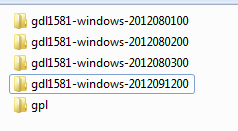
\includegraphics{../images/gendl-installation.png}
\end{center}

\caption{Several Gendl versions and one GPL }

\label{fig:gendl-installation}

\end{figure}
So you now should have two directories at the same level: one named \texttt{gdl1581.../}(the rest of the name will contain the specific dated build stamp), and a \texttt{gdl/}directory at the same level. Note that as seen in Figure 
\ref{fig:gendl-installation}, it is possible to have several Gendl versions installed, but just a single common \texttt{gpl/} folder.

\subsection{Test your Installation}

\label{subsec:testyourinstallation}

Test your installation according to the following checklist:

\begin{enumerate}

\item Invoke the \texttt{run-gdl.bat} (Windows), or \texttt{run-gdl} (Linux, MacOS) startup script. This should launch Gnu Emacs with a 
README file displayed by default. Take the time to look through this README file. 
Especially the later part of the file contains information about Emacs keyboard
shortcuts available.

\item In emacs, enter: \texttt{M-x glime}. That is, hold down the ``Meta'' (or ``Alt'') key, and press the ``M'' key. 
You will see this command shown in the \emph{mini-buffer} at the bottom of the Emacs window, as shown in Figure 
\ref{fig:mini-buffer}

\item press the ``Enter'' key

\item On Windows, you will get a new window, named the Allegro CL Console or the Gendl Console. 
Watch this console for any errors or warnings. 

The first time you start up, you may see messages in this console for
several minutes while the system is being built (or if you received a
completely pre-built system, the messages may last only a few
seconds).

On Linux or MacOS, there will be a separate Emacs buffer (available
through Emacs' ``Buffers'' menu) where you will see these messages.

The messages will consist of compiling and loading information, followed by copyright and welcome information
for Gendl. After these messages have finished, you should see the following command prompt:\texttt{gdl-user(1): }

\item In your Web Browser (e.g. Google Chrome, Firefox, Safari, Opera, Internet Explorer), 
perform the following steps:

\begin{enumerate}

\item visit http://localhost:9000/tasty.

\item accept default robot:assembly.

\item Select ``Add Leaves'' from the Tree menu.

\item Click on the top node in the tree.

\item Observe the wireframe graphics for the robot.

\item Click on the robot to zoom in.

\item Select ``Clear View!'' from the View menu.

\item Select ``X3DOM'' from the View menu.

\item Click on the top node in the tree.

\item ``Refresh'' or ``Reload'' your browser window (may not be necessary).
\item If your browser supports WebGL, you will see the robot in shaded dynamic view.

\item Select ``PNG'' from the View menu.

\item You will see the wireframe view of the robot as a PNG image.


\end{enumerate}



\end{enumerate}



\subsection{Make a Desktop Shortcut}

\label{subsec:makeadesktopshortcut}



\subsection{Populate your Initialization File}

\label{subsec:populateyourinitializationfile}

The default initialization file for Gendl is called 
\tt{gdlinit.cl}, 

\section{Installation of open-source Gendl}

\label{sec:installationofopen-sourcegendl}



\subsection{Install and Configure your Common Lisp environment}

\label{subsec:installandconfigureyourcommonlispenvironment}

Gendl is currently tested to build on the following Common Lisp engines:

\begin{itemize}

\item Allegro CL (commercial product from Franz, free Express Edition available)

\item LispWorks (commercial product from LispWorks Ltd, free Personal Edition available)

\item Steel Bank Common Lisp (SBCL) (free open-source project with permissive license)

\end{itemize}

Please refer to the documentation for each of these systems for full information on installing 
and configuring the environment. Typically this will include a text editor, either Gnu Emacs with Superior
Lisp Interaction Mode for Emacs (Slime), or a built-in text editing and development environment which 
comes with the Common Lisp system.

\backmatter



\printindex



\end{document}

